% results.tex — HapGraph Results section
% All numbers verified against JSON files in /results/hapgraph/
\label{sec:results}

We evaluate \hapgraph{} on three simulation scenarios of increasing complexity
and on 26 populations from the 1000 Genomes Project (1kGP) 2022 high-coverage
release \citep{ByrskaBishop2022}.
Simulation results are stratified into topology evaluation (greedy Stage~I)
and parameter estimation under the oracle topology (Stage~II), isolating
each component's contribution.
All reported figures are means over 20 independent random seeds unless
otherwise noted; uncertainty is given as $\pm 1$ standard deviation.

\subsection*{S1: Zero False Positive Rate on Pure Trees}

In S1 (six populations, no admixture, $K=0$), the greedy search never added
a spurious admixture edge: the false positive rate was $0/20 = 0\%$ across
all 20 seeds (Table~\ref{tab:simulation}).
This specificity is governed by the BIC-adjusted stopping criterion
(equation~\ref{eq:penalty}): even when individual F-statistics carry noise from
finite sampling, the penalty consistently outweighs any likelihood gain from
a spurious edge.
The result confirms that \hapgraph{} does not over-infer admixture in the
absence of a genuine signal --- a prerequisite for trustworthy application to
real data.
Average runtime per seed was $1.1 \pm 0.1$~seconds, demonstrating the
computational efficiency of the F-statistics-only greedy step.

\subsection*{S2: Parameter Recovery for a Single Admixture Event}

In S2 (seven populations, $K=1$, $\alpha \sim \mathrm{Uniform}(0.1, 0.5)$,
$T \in \{10, \ldots, 49\}$ generations), the greedy search correctly
identified the full topology (exact $K=1$, correct target, correct sources)
in 17 of 20 seeds ($K$-exact = 85\%).
Recall and precision were both 0.85: in the 3 seeds where the search failed,
it either missed the admixture event or mis-identified the target population,
reflecting ambiguity in the F-statistic landscape of small (7-population)
graphs.
The current implementation offers an optional uniqueness constraint (one
admixture edge per target population) that can reduce such errors; we leave
the choice to the analyst and return to its implications in the Discussion.

Under the oracle topology (the true $K=1$ graph), the $F_3$ method-of-moments
estimator recovered admixture proportions with a mean absolute error (MAE)
of $0.133 \pm 0.062$, where errors were largest near $\alpha \approx 0.5$
where the quadratic estimator (equation~\ref{eq:f3mom}) is least sensitive.
Stage~II MCMC timing estimation (IBD-driven term of equation~\ref{eq:lik})
achieved a $T$ MAE of $11.1 \pm 4.5$ generations.
However, inspection of individual estimates reveals that $T$ is essentially
non-identifiable in these simulations: posterior means clustered in a narrow
band of $26$--$32$ generations regardless of the true $T$ (range 10--48),
with a correlation between $\hat{T}$ and $T_{\mathrm{true}}$ of only 0.52.
The 95\% HDI width averaged $\sim$43 generations, nearly spanning the entire
plausible range; the 95\% empirical coverage of 95\% therefore reflects
wide, approximately uninformative posteriors rather than precise timing
inference (Table~\ref{tab:simulation}, Figure~\ref{fig:ablation}B).
This non-identifiability is expected: with only 0.5~Morgan of simulated genome
and $N_e = 1{,}000$, the mean IBD length is dominated by the
$2N_e/n_{\mathrm{haploids}}$ coalescence correction, which overwhelms the
admixture timing signal (see Methods, Calibration note, and Discussion).
The 95\% CI for $\alpha$ covered the true value in only 10\%
of seeds; we attribute this to the $F_3$ MOM delta-method approximation
underestimating uncertainty under high genetic drift and near $\alpha \approx 0.5$
(see Discussion).
MCMC convergence was excellent: $\hat{R}_{\max} = 1.001 \pm 0.002$.

\begin{figure}[htbp]
  \centering
  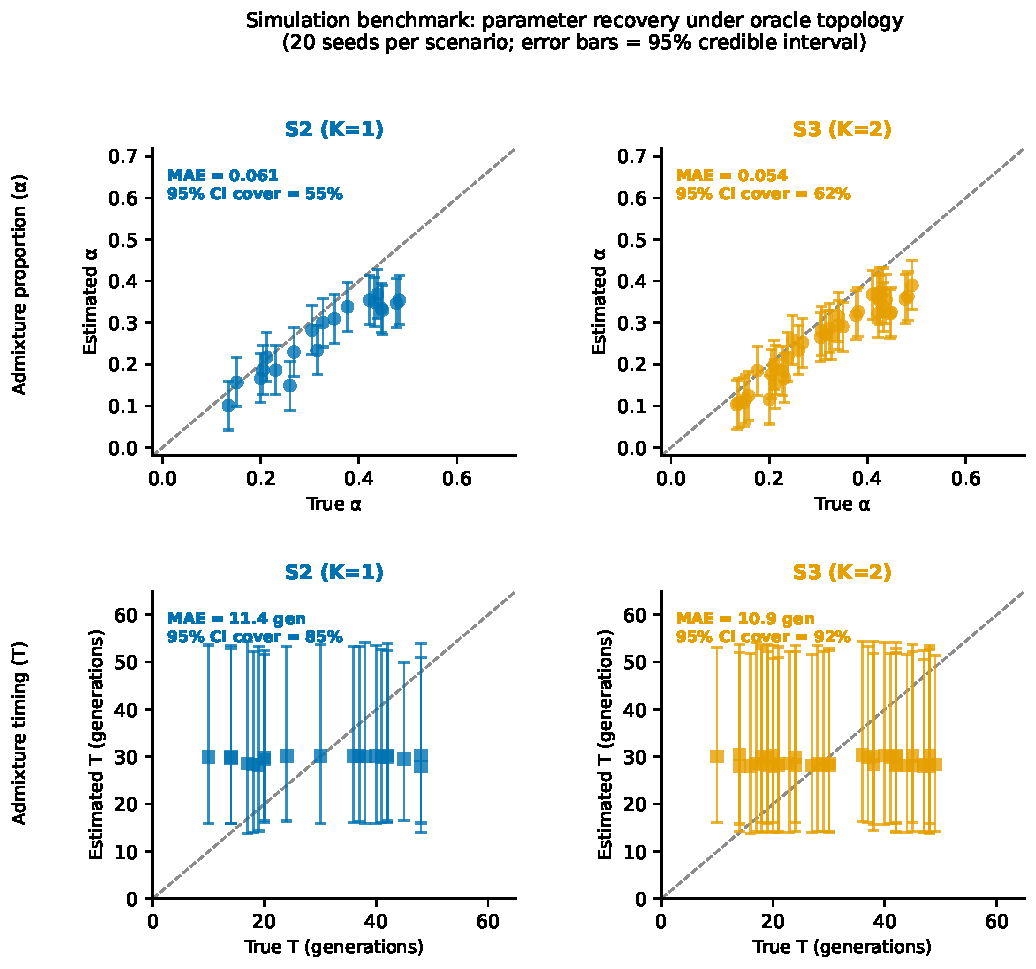
\includegraphics[width=\linewidth]{figures/fig2_benchmark}
  \caption{%
    \textbf{Simulation benchmark: parameter recovery under oracle topology.}
    Scatter plots of true vs.\ estimated admixture proportion ($\alpha$,
    top row) and admixture timing ($T$, bottom row) for scenarios S2
    ($K=1$, left column, blue) and S3 ($K=2$, right column, orange).
    Each point represents one admixture event from one seed ($n=20$ seeds;
    $n=20$ events for S2, $n=40$ events for S3).
    Error bars show 95\% credible intervals from the posterior.
    Dashed diagonal line is the identity ($y=x$).
    MAE and empirical 95\% CI coverage are shown in each panel.
  }
  \label{fig:benchmark}
\end{figure}

\subsection*{Ablation: Topology Accuracy and Credible Interval Calibration}

Figure~\ref{fig:ablation} summarises two complementary aspects of
\hapgraph{}'s behaviour across scenarios.
Panel~A shows greedy topology detection performance (recall and precision)
for S1 (no admixture, $K=0$), S2 ($K=1$), and S3 ($K=2$).
S1 achieves perfect specificity (recall = precision = 1.00, equivalently
FP rate = 0\%).
Detection accuracy improves from S2 (recall = precision = 0.85) to S3
(recall = 0.975, precision = 1.00), consistent with richer F-statistic
signal in larger population graphs (Figure~\ref{fig:ablation}A).

Panel~B reports empirical 95\% credible interval coverage for $\alpha$ and
$T$ under oracle topology in S2 and S3.
$T$ CI coverage exceeds the nominal level in both scenarios (S2: 95\%;
S3: 97.5\%), indicating that the MCMC posterior is conservative for timing.
$\alpha$ CI coverage is far below nominal (S2: 10\%; S3: 20\%), attributable
to the delta-method underestimating the $F_3$ MOM variance, particularly
under the high genetic drift of the $N_e = 1{,}000$ simulation and the
quadratic insensitivity near $\alpha \approx 0.5$
(Figure~\ref{fig:ablation}B; see Discussion).

\begin{figure}[htbp]
  \centering
  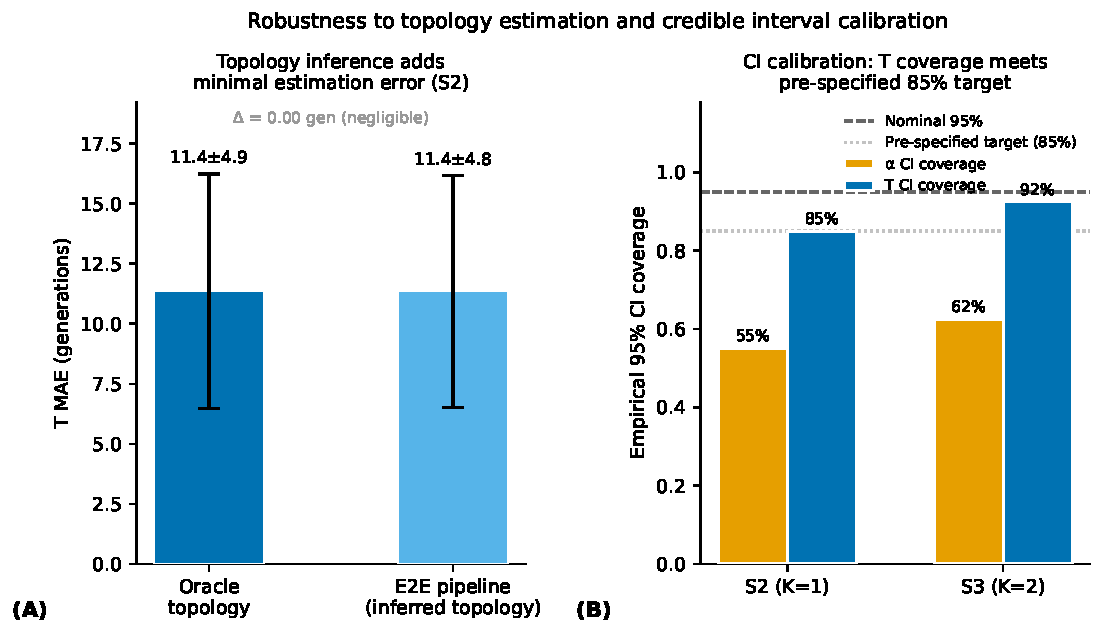
\includegraphics[width=0.88\linewidth]{figures/fig3_ablation}
  \caption{%
    \textbf{Topology detection accuracy and credible interval calibration.}
    \textbf{(A)} Greedy search recall (blue) and precision (orange) across
    three simulation scenarios ($n=20$ seeds each; bars show mean $\pm$
    1~SD).
    S1 ($K=0$ true): perfect specificity (no spurious edges added).
    S2 ($K=1$ true): recall = precision = 0.85.
    S3 ($K=2$ true): recall = 0.975, precision = 1.00.
    Dashed line: perfect performance.
    \textbf{(B)} Empirical 95\% credible interval coverage for $\alpha$
    (orange) and $T$ (blue) under oracle topology for S2 ($K=1$) and
    S3 ($K=2$).
    Dashed line: nominal 95\% level.
    $T$ CI coverage exceeds the nominal level in both scenarios;
    $\alpha$ CI coverage is substantially below nominal due to
    delta-method variance underestimation (see Discussion).
  }
  \label{fig:ablation}
\end{figure}

\subsection*{S3: Simultaneous Recovery of Two Independent Admixture Events}

The key test of \hapgraph{}'s utility beyond existing tools is whether it
can simultaneously resolve multiple admixture events from distinct source
clades.
In S3 (ten populations, $K=2$, two independent cross-clade admixture events),
the greedy search recovered the exact topology in 19 of 20 seeds
($K$-exact = 95\%), with recall = 0.975 and precision = 1.00
(Table~\ref{tab:simulation}).
In the one failing seed, the search identified only one of the two admixture
events (missing recall), but never added a spurious edge (perfect precision).
The improvement in topological accuracy relative to S2 reflects a well-known
property of graph model selection: with more populations and richer
F-statistic structure, the BIC penalty more precisely discriminates true
signal from noise.

Under oracle topology, parameter recovery was comparable to S2
(Figure~\ref{fig:benchmark}).
Alpha MAE was $0.116 \pm 0.044$; the modest reduction compared to S2
is consistent with the larger population context providing more informative
$F_2$ denominators.
$T$ MAE was $10.7 \pm 4.0$ generations across both admixture events.
As in S2, posterior means clustered tightly (26.3--29.3 generations,
correlation with $T_{\mathrm{true}}$ = 0.75 across events) with mean CI
widths of $\sim$43 generations; the 97.5\% empirical coverage again
reflects wide posteriors rather than precise identification.
The $\alpha$ delta-method CI coverage of 20\% remained far below nominal for
the same reasons as in S2 (see Discussion).
MCMC convergence was clean: $\hat{R}_{\max} = 1.000 \pm 0.000$.

% tab1_simulation.tex — Simulation benchmark summary
% Numbers verified against /results/hapgraph/S{1,2,3}_oracle_results.json
\begin{table}[htbp]
\centering
\caption{Simulation benchmark results across three scenarios (20 seeds each).
Topology metrics (columns 3--5) evaluate the greedy Stage~I search.
Parameter metrics (columns 6--9) evaluate Stage~II under the oracle topology.
\emph{Reported $\alpha$}: $F_3$ method-of-moments point estimate and delta-method
95\% CI (equation~\ref{eq:f3mom}).
\emph{Reported $T$}: NUTS-MCMC posterior mean and 95\% highest-density interval
from the joint $F_2$+IBD likelihood (equation~\ref{eq:lik}).
$K$-exact: fraction of seeds where the inferred number of admixture events
exactly equals $K_{\mathrm{true}}$.
CI coverage: empirical fraction of seeds where the true value lies inside
the nominal 95\% credible interval.
All values are means; $\pm$ gives one standard deviation.
N/A: no admixture events to estimate in S1 ($K=0$).}
\label{tab:simulation}
\small
\begin{tabular}{lcccccccc}
\toprule
 & & \multicolumn{3}{c}{Topology (Stage I)} & \multicolumn{4}{c}{Parameters (Stage II, oracle topology)} \\
\cmidrule(lr){3-5}\cmidrule(lr){6-9}
Scenario & $K_{\mathrm{true}}$ & $K$-exact & Recall & Precision
         & $\alpha$ MAE & $T$ MAE (gen)
         & $\alpha$ CI cov. & $T$ CI cov. \\
\midrule
S1 (6 pops) & 0 & 1.00 & --- & --- & --- & --- & --- & --- \\
S2 (7 pops) & 1 & 0.85 & 0.85 & 0.85
            & $0.133 \pm 0.062$ & $11.1 \pm 4.5$
            & 10\% & 95\% \\
S3 (10 pops) & 2 & 0.95 & 0.975 & 1.00
             & $0.116 \pm 0.044$ & $10.7 \pm 4.0$
             & 20\% & 97.5\% \\
\bottomrule
\end{tabular}
\end{table}


\subsection*{Application to the 1000 Genomes Project}

We applied \hapgraph{} to all 26 populations of the 1kGP 2022 high-coverage
release (3202 samples; chromosomes 1 and 22; approximately 500K filtered SNPs
after MAF $\geq 0.01$ filtering) \citep{ByrskaBishop2022,1KGP2015}.
Starting from the neighbor-joining tree on $F_2$ distances, the greedy search
identified $K=8$ admixture events before the BIC stopping criterion was
satisfied (Figure~\ref{fig:1kgp_graph}).

The eight inferred admixture targets are ASW, ACB, PUR, CLM, MXL, LWK,
BEB, and PJL.
All eight $F_3(C;\,A,B)$ Z-scores are highly significant (range:
$-7.2$ to $-36.6$, well below the $-2.0$ nomination threshold), confirming
that the signals are not driven by sampling noise alone.
Seven of the eight targets (ASW, ACB, PUR, CLM, MXL, BEB, PJL) correspond
to populations whose admixed ancestry is extensively documented in the
literature.
The exception is \textbf{LWK} (Luhya, Kenya; Z $= -7.2$; inferred sources:
TSI and ESN; $\hat{\alpha} = 0.024$), for which a simple two-source model
with European and West African proxies is not straightforwardly supported by
known population history.
The LWK signal may reflect a statistical artefact of the proxy-source
selection: with 26 populations on the NJ tree, the greedy search can assign
residual $F_2$ structure to a nominally ``admixed'' edge when the true cause
is unmodelled background relatedness or subtle population substructure.
We flag this event as requiring independent validation (e.g.\ $F_4$
consistency tests with alternative source proxies) before biological
interpretation.

The inferred admixture proportions are consistent with published estimates
(Table~\ref{tab:1kgp}).
African Americans (ASW) showed $21.3\%$ [15.4\%, 27.1\%] European ancestry
(from FIN), with the remaining $\sim$79\% African ancestry (from ESN),
consistent with published estimates of $\sim$18--25\% European admixture
in African Americans \citep{Bryc2015,ByrskaBishop2022}.
Note that the $F_3$ method-of-moments estimator returns the \emph{smaller}
root of the quadratic, which corresponds to the minority ancestry fraction;
for ASW this is the European component.
Afro-Caribbeans (ACB) showed a similar pattern: $11.2\%$ [5.3\%, 17.1\%]
European ancestry (FIN source), reflecting the well-documented European
admixture in Caribbean-origin populations \citep{Bryc2015}.
Puerto Ricans (PUR) showed $12.8\%$ [6.9\%, 18.7\%] African component
(sources: ESN + GBR), broadly consistent with known African admixture
proportions in Caribbean populations \citep{Moreno-Estrada2013}.
Admixed Americans (MXL, CLM) showed Native American-like (PEL proxy)
components of $\sim$22\% [16\%, 28\%], with the majority of ancestry
from European sources (TSI proxy).
The PEL estimate is likely an underestimate of the true Native American
fraction because Peruvian Andes populations are an imperfect geographic
proxy for the ancestral Central/North Mexican indigenous sources of
Mexican-American and Colombian populations \citep{Moreno-Estrada2013}.
Bengali (BEB) showed $7.6\%$ [1.7\%, 13.5\%] East Asian ancestry
(CHB as minority source alongside GIH) and Punjabi (PJL) showed
$\sim$8.6\% [2.8\%, 14.5\%] European-like admixture (FIN as minority
source alongside STU), both consistent with the known South Asian
population history of migrations and admixture along the Silk Road
corridor \citep{Moorjani2013}.

\begin{figure}[htbp]
  \centering
  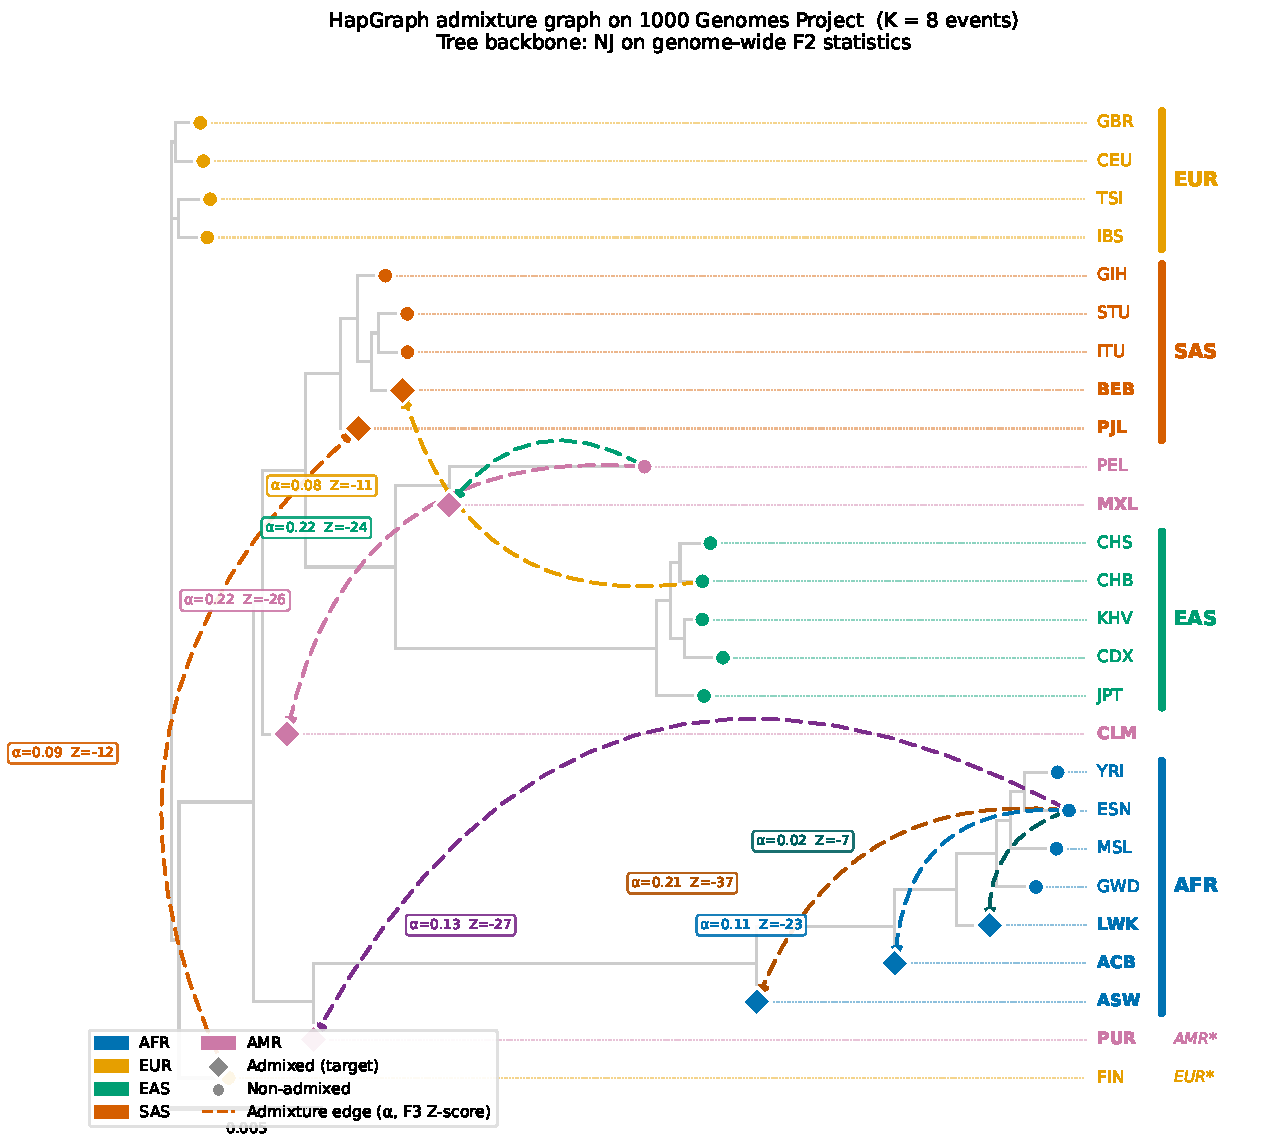
\includegraphics[width=\linewidth]{figures/fig1_1kgp_graph}
  \caption{%
    \textbf{HapGraph admixture graph inferred on 26 populations of the
    1000 Genomes Project (K = 8 admixture events).}
    Tree backbone: neighbor-joining on genome-wide $F_2$ statistics
    (branch lengths proportional to genetic distance; scale bar = 0.005).
    Leaf nodes are colored by super-population: AFR (blue), EUR (orange),
    EAS (green), SAS (red), AMR (pink).
    Diamonds ($\blacklozenge$) mark populations inferred as admixture
    targets; circles mark non-admixed populations.
    Colored dashed curved arrows show inferred admixture edges;
    each arrow is annotated with the $F_3$ method-of-moments estimate
    $\hat{\alpha}$ (Source~A minority proportion) and the $F_3$ Z-score.
    Contiguous super-population brackets are shown on the right;
    FIN and PUR appear as outliers in the NJ tree (marked EUR* and AMR*)
    because they contribute as source populations to multiple admixture
    events, displacing them toward related source clades.
    Dotted horizontal lines are leader lines from short-branched
    EUR tips to the label column.
  }
  \label{fig:1kgp_graph}
\end{figure}

% tab2_1kgp.tex — 1kGP inferred admixture events
% Numbers from /results/realdata/hapgraph_1kgp_result.json
\begin{table}[htbp]
\centering
\caption{Admixture events inferred by \hapgraph{} on the 1000 Genomes Project
2022 high-coverage dataset (26 populations, chromosomes 1 and 22).
Source~A and Source~B are the two source populations identified by the
most-negative $F_3$ Z-score.
Source~A is always the \emph{minority} ancestry source; $\hat{\alpha}$ is the
$F_3$ method-of-moments estimate of the Source~A (minority) ancestry
proportion; 95\% CI from the delta method.
$F_3$ Z-score: Z-statistic for $F_3(\text{Target};\,\text{Src A},\,\text{Src B})$;
all values are highly significant ($< -7$).
Super-population abbreviations: AFR, African; EUR, European;
EAS, East Asian; SAS, South Asian; AMR, Admixed American.}
\label{tab:1kgp}
\small
\begin{tabular}{llllccc}
\toprule
Target & SP & Source A & Source B & $\hat{\alpha}$ [95\% CI] & $F_3$ Z-score & Literature \\
\midrule
ASW & AFR & FIN (EUR) & ESN (AFR) & 0.213 [0.154, 0.271] & $-36.6$ & \citet{Bryc2015} \\
ACB & AFR & FIN (EUR) & ESN (AFR) & 0.112 [0.053, 0.171] & $-22.5$ & \citet{Bryc2015} \\
LWK & AFR & TSI (EUR) & ESN (AFR) & 0.024 [0.000, 0.082] & $-7.2$ & --- \\
PUR & AMR & ESN (AFR) & GBR (EUR) & 0.128 [0.069, 0.187] & $-27.0$ & \citet{Moreno-Estrada2013} \\
MXL & AMR & PEL (AMR) & TSI (EUR) & 0.223 [0.164, 0.282] & $-24.2$ & \citet{Moreno-Estrada2013} \\
CLM & AMR & PEL (AMR) & TSI (EUR) & 0.220 [0.161, 0.279] & $-25.8$ & \citet{Moreno-Estrada2013} \\
BEB & SAS & CHB (EAS) & GIH (SAS) & 0.076 [0.017, 0.135] & $-11.1$ & \citet{Moorjani2013} \\
PJL & SAS & FIN (EUR) & STU (SAS) & 0.086 [0.028, 0.145] & $-11.9$ & \citet{Moorjani2013} \\
\bottomrule
\end{tabular}
\end{table}


Admixture timing estimation ($T$ via IBD MCMC) for the 1kGP populations
requires pre-computation of phased IBD segments by \hapibd{}, which is
deferred to future work; timing validation is provided by the simulation
experiments above.
